
%(BEGIN_QUESTION)
% Copyright 2010, Tony R. Kuphaldt, released under the Creative Commons Attribution License (v 1.0)
% This means you may do almost anything with this work of mine, so long as you give me proper credit

Suppose we had a single-ported globe valve such as this controlling fluid flow, with inlet and outlet pressures as shown in the illustration.  If the plug has a cross-sectional area of 20 cm², how much force will be exerted on the plug by the fluid?  In which direction will this force be exerted?

$$\includegraphics[width=8.5cm]{i00772x01.eps}$$

\filbreak

Now suppose we replace the single-ported globe valve with a {\it double-ported} globe valve of similar operating characteristics.  Given the same inlet and outlet pressures, how much (net) force will be exerted on the plugs by the fluid?  Assume the upper plug has a cross-sectional area of 20 cm² , and the lower plug a cross-sectional area of 13 cm²:

$$\includegraphics[width=8.5cm]{i00772x02.eps}$$

Which of these two control valves will be easier to position (i.e. require less actuating force), all other factors being equal?

\vskip 20pt \vbox{\hrule \hbox{\strut \vrule{} {\bf Suggestions for Socratic discussion} \vrule} \hrule}

\begin{itemize}
\item{} For the valve requiring less actuating force, are there any disadvantages to the design?  Clearly, lower actuating force is a good thing, so there must be some drawback to this design or else {\it all} control valves would be manufactured this way!
\item{} Is the direction of flow arbitrary for this control valve, or is there a reason why the flow should be passing {\it up} past the plug rather than {\it down} past it?
\item{} Does the packing of a double-ported control valve need to be different than the packing of a single-ported valve?  Why or why not?
\end{itemize}

\underbar{file i00772}
%(END_QUESTION)





%(BEGIN_ANSWER)

For the single-ported valve, the force will be 150 lbs in the upward direction.  For the double-ported valve, the force will be substantially less.

%(END_ANSWER)





%(BEGIN_NOTES)

For the single-ported valve, the force will be 150 lbs in the upward direction.  For the double-ported valve, the force will be only 50 lbs in the upward direction.









\vfil \eject

\noindent
{\bf Prep Quiz:}

An inherent advantage of double-ported globe valves over single-ported globe valves is:

\begin{itemize}
\item{} Tighter shut-off due to fewer places for process fluid to leak
\vskip 5pt 
\item{} Less actuating force required to overcome process fluid forces
\vskip 5pt 
\item{} Longer service life due to harder seat materials used
\vskip 5pt 
\item{} Less friction along the valve stem caused by fluid leakage
\vskip 5pt 
\item{} Less expensive to purchase and less bulky to store spare parts
\vskip 5pt 
\item{} Easier to rebuild, due to less complex design and construction
\end{itemize}

%INDEX% Final Control Elements, valve: dynamic fluid force on globe valve plug
%INDEX% Final Control Elements, valve: double-ported
%INDEX% Final Control Elements, valve: single-ported

%(END_NOTES)


